\documentclass[]{book}
%\usepackage{setspace}
%\onehalfspacing
\usepackage{amsmath,amssymb,amsthm}
\renewcommand{\qedsymbol}{$\blacksquare$}
\usepackage{amsmath}
\usepackage{amsfonts}
\usepackage{mathrsfs}
\usepackage{amssymb}
\usepackage{enumerate}
\usepackage{mdwlist}
\usepackage{dirtytalk}
\usepackage{xparse}
\usepackage{physics}
\usepackage{graphicx}
\setcounter{MaxMatrixCols}{13}
\setlength\parindent{0pt}
\usepackage[none]{hyphenat}
\usepackage[hmarginratio=1:1]{geometry}
\begin{document}
\begin{center}
{\Large Physics 622 Homework 8}\\
{Jeremy Welsh-Kavan}\\
\end{center}
\vspace{0.2 cm}
\begin{center}
\noindent\rule{15cm}{0.4pt} \\
\end{center}
My homework in LaTex, as requested. I pray it pleases thee, exalted grader. \\
\vspace{0.1 cm} \\
{2.2.3 \hspace{0.5cm} \textbf{Electrostatics in $d$ dimensions (continued)}} \\
\vspace{0.1 cm} \\
\textbf{b)} We calculate and plot the potential $\varphi$ and the field $\textbf{E}$ for $d=2$, for the case of a homogeneously charged disk, $\rho(\textbf{x}) = \rho_0 \Theta(r_0-|\textbf{x}|)$. \\
For $d=2$, the $\textbf E$ field and the potential satisfy

\begin{equation}
\textbf{E}(\textbf{x}) = - \nabla\varphi(\textbf{x})
\end{equation}
and 
\begin{equation}
\nabla^2\varphi(\textbf{x}) = -2 \pi\rho(\textbf{x})
\end{equation}
Since $\rho(\textbf{x})$ is azimuthally symmetric, we know that $\varphi(\textbf{x})$ will be azimuthally symmetric. In this case, we can rewrite (2) as
\begin{equation}
\frac{1}{r}\pdv{r}\left( r\pdv{r}\varphi(r)\right) = -2\pi\rho_0 \Theta(r_0-r)
\end{equation}
From this we can directly solve for $\varphi(r)$ by integrating (3) twice.
\begin{equation}
\begin{split}
r\pdv{r}\varphi(r) & = -2\pi\rho_0 \int dr \text{ } r \Theta(r_0-r) \\
r\pdv{r}\varphi(r) & = -2\pi\rho_0 \begin{cases}
\frac{r^2}{2}, \text{ } 0\leq r\leq r_0 \\
\frac{r_0^2}{2}, \text{ }r>r_0 \\
\end{cases} \\
\pdv{r}\varphi(r) & = -\pi\rho_0 \left( r + \Theta(r-r_0)(\frac{r_0^2}{r} - r)\right) \\
\varphi(r) & = -\pi\rho_0\left( \frac{r^2}{2} +  \Theta(r-r_0)\left( \frac{r_0^2}{2} - \frac{r^2}{2} + r_0^2\text{ln}\left( \frac{r}{r_0}\right) \right) \right) \\
\text{or} \\
\varphi(r) & = -\pi\rho_0 \begin{cases}
\frac{r^2}{2}, \text{ } 0\leq r\leq r_0 \\
\frac{r_0^2}{2} + r_0^2\text{ln}\left( \frac{r}{r_0}\right), \text{ } r_0 < r \\
\end{cases}
\\
\end{split}
\end{equation}
\\
Finally, we can redefine $\varphi(r_0)=0$ to get
\begin{equation}
\varphi(r) = \begin{cases}
\pi\rho_0\left( \frac{r_0^2}{2} - \frac{r^2}{2} \right) , 0\leq r\leq r_0 \\
\pi\rho_0 r_0^2 \text{ln}\left( \frac{r_0}{r}\right), \text{ } r_0 < r \\
\end{cases}
\end{equation}
We find the $\textbf{E}$ field by taking the negative gradient of (5).
\begin{equation}
\begin{split}
\textbf{E}(\textbf{x}) &= - \nabla\varphi(\textbf{x}) \\
\textbf{E}(\textbf{x}) &= - \pdv{\varphi(r)}{r}\hat{e}_r \\
\textbf{E}(\textbf{x}) &= E(r)\hat{e}_r \\
E(r) & = \begin{cases}
\pi\rho_0r  , 0\leq r\leq r_0 \\
\pi\rho_0 \frac{r_0^2}{r}, \text{ } r_0 < r \\
\end{cases}
\end{split}
\end{equation}

\begin{frame}{}
    \begin{figure}[h]
        \begin{minipage}[b]{0.5\linewidth}
            \centering
            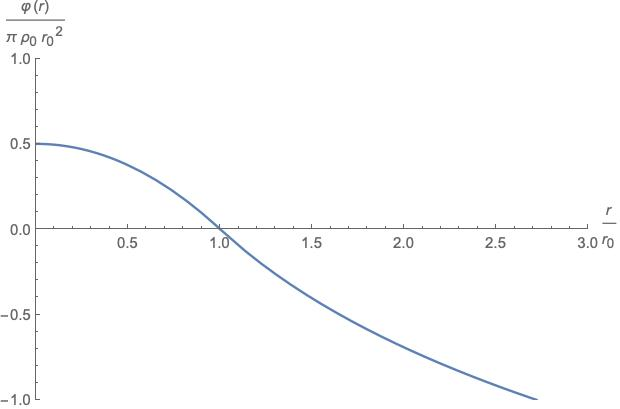
\includegraphics[width=\textwidth]{2Ddiscpotential.jpeg}
        \end{minipage}
        \hspace{0.5cm}
        \begin{minipage}[b]{0.5\linewidth}
            \centering
            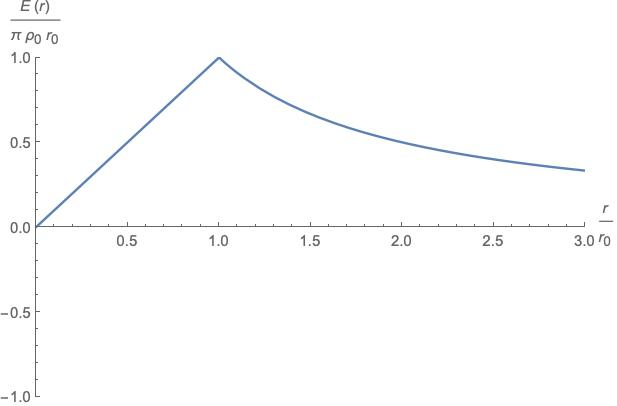
\includegraphics[width=\textwidth]{2DdiscEfield.jpeg}
        \end{minipage}
        \caption{Plots of the potential, $\varphi(r)$, and the radial component of the electric field, $E(r)$, in convenient units.}
    \end{figure}
\end{frame}

\textbf{c)} We proceed as above, but for d=1. Here, d=1 and $\rho(x) = \rho_0\Theta(x_0^2/4-x^2)$, which represents the charge density of a uniformly charged rod of length $x_0$ centered at the origin. In the d=1 case, $\textbf{E}(\textbf{x})$ and $\varphi(x)$ are both just scalar fields given by the equations
\begin{equation}
\begin{split}
\pdv{E(x)}{x} &= 2\rho(x)\\
\pdv[2]{\varphi(x)}{x} & = -2\rho(x)\\
\end{split}
\end{equation}
Solving for $E(x)$, we have
\begin{equation}
\begin{split}
\pdv{E(x)}{x} &= 2\rho_0\Theta\left(1 - \frac{4x^2}{x_0^2}\right)\\
E(x) & = \begin{cases}
-\rho_0x_0, \text{ } x< -\frac{x_0}{2} \\
2\rho_0x, \text{ }  -\frac{x_0}{2} \leq x \leq  \frac{x_0}{2} \\
\rho_0x_0, \text{ } \frac{x_0}{2} <x\
\end{cases}
\end{split}
\end{equation}
We can define $\varphi(\frac{x_0}{2})=0$, and since the potential is symmetric is the charge distribution is symmetric, $\varphi(-\frac{x_0}{2})=0$ as well. To obtain $\varphi(x)$ we integrate (8), which yields
\begin{equation}
\begin{split}
\varphi(x) & = -\int_{x_0/2}^{x}dxE(x)\\
\varphi(x) & = 
\begin{cases}
\rho_0x_0x + \frac{\rho_0x_0^2}{2}, \text{ } x< -\frac{x_0}{2} \\
\frac{\rho_0x_0^2}{4}-\rho_0x^2, \text{ } -\frac{x_0}{2} \leq x \leq  \frac{x_0}{2} \\
-\rho_0x_0x + \frac{\rho_0x_0^2}{2}, \text{ } \frac{x_0}{2}<x \\
\end{cases}
\end{split}
\end{equation}
\begin{frame}{}
    \begin{figure}[h]
        \begin{minipage}[b]{0.5\linewidth}
            \centering
            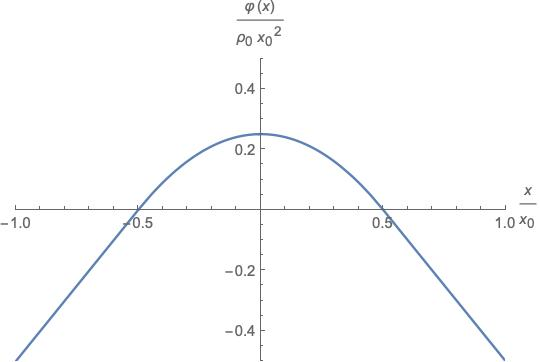
\includegraphics[width=\textwidth]{1Drodpotential.jpeg}
        \end{minipage}
        \hspace{0.5cm}
        \begin{minipage}[b]{0.5\linewidth}
            \centering
            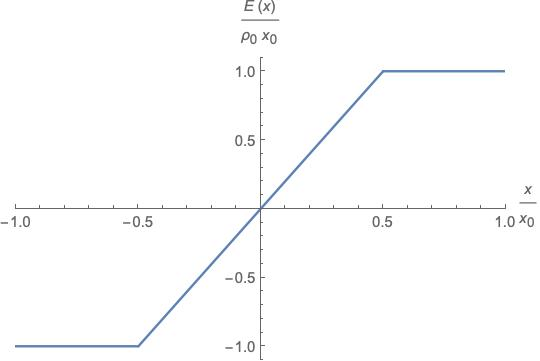
\includegraphics[width=\textwidth]{1DrodEfield.jpeg}
        \end{minipage}
        \caption{Plots of the potential, $\varphi(x)$, and the electric field, $E(x)$, in convenient units.}
    \end{figure}
\end{frame}
\\
\\
\\
\noindent\rule{15cm}{0.4pt} \\

{2.2.4 \hspace{0.5cm} \textbf{Helmholtz Equation}} \\
\vspace{0.1 cm} \\
Our goal is to find the most general Fourier transformable solution, $\varphi(\textbf{x})$, to the Helmholtz equation,
\begin{equation}
\left(\kappa^2-\nabla^2\right)\varphi(\textbf{x})=4\pi\rho(\textbf{x})
\end{equation}
We can begin by funding the fundamental solution, $G(\textbf{x})$, of the Helmholtz operator. That is, a function, $G(\textbf{x})$ satisfying
\begin{equation}
\left(\kappa^2-\nabla^2\right)G(\textbf{x})=-4\pi\delta(\textbf{x})
\end{equation}
Taking the Fourier transform of both sides of (6) gives
\begin{equation}
\begin{split}
\frac{1}{(\sqrt{2\pi})^3}\int d^3\textbf{x}\left(\kappa^2-\nabla^2\right)G(\textbf{x}) e^{-i \textbf{k}\cdot\textbf{x}} &=-\frac{4\pi}{(\sqrt{2\pi})^3} \\
(\kappa^2+ \textbf{k}^2)\hat{G}(\textbf{\textbf{k}}) &= -\sqrt{\frac{2}{\pi}} \\
\hat{G}(\textbf{\textbf{k}}) &= -\sqrt{\frac{2}{\pi}} \frac{1}{\textbf{k}^2+ \kappa^2}
\end{split}
\end{equation}
We now inverse Fourier transform the last line of (7) to get
\begin{equation}
\begin{split}
G(\textbf{x}) &= -\sqrt{\frac{2}{\pi}} \frac{1}{(\sqrt{2\pi})^3} \int d^3\textbf{k}\text{ } \frac{e^{i \textbf{k}\cdot\textbf{x}}}{\textbf{k}^2+ \kappa^2}
\end{split}
\end{equation}
which we can compute in spherical coordinates as follows:
\begin{equation}
\begin{split}
G(\textbf{x}) &= -\frac{1}{2\pi^2} \int_{0}^{\infty}\int_{0}^{2\pi}\int_{0}^{\pi} \frac{e^{ir|\textbf{x}|\text{cos}\theta}}{r^2+ \kappa^2}  r^2 \text{sin}\theta d\theta d\phi dr\\
G(\textbf{x}) &= -\frac{1}{\pi} \int_{0}^{\infty}\int_{0}^{\pi} \frac{e^{ir|\textbf{x}|\text{cos}\theta}}{r^2+ \kappa^2}  r^2 \text{sin}\theta d\theta dr \\
G(\textbf{x}) &= -\frac{2}{\pi |\textbf{x}|}\int_{0}^{\infty} \frac{r\text{ }\text{sin}(r|\textbf{x}|)}{r^2+ \kappa^2} dr \\
G(\textbf{x}) &= -\frac{e^{-\kappa|\textbf{x}|}}{|\textbf{x}|} \\
\end{split}
\end{equation}
Where the last integral in (9) can be computed with Mathematica or using the residue theorem. Note that this differs by a sign from the Green's function of the Laplacian that we found in 2.2.3 a) since the Laplacian carries a minus sign in the Helmholtz equation. With $G(\textbf{x})$,we can find a general expression for $\varphi(\textbf{x})$. From what we know about Green's functions, if $\varphi(\textbf{x})$ satisfies (5), then we can express $\varphi(\textbf{x})$ in terms of a convolution with $G(\textbf{x})$. Just to convince ourselves that this makes sense, below is some hand-wavy algebra. Let $L = \kappa^2-\nabla^2$. If $G(\textbf{x})$ satisfies
\begin{equation}
L\left[G(\textbf{x}-\textbf{y})\right] = -4\pi\delta^3(\textbf{x}-\textbf{y})
\end{equation}
then we have \\
\begin{equation}
\begin{split}
\int d^3\textbf{y} L\left[G(\textbf{x}-\textbf{y})\right] \rho(\textbf{y}) &= -4\pi \int d^3\textbf{y} \delta^3(\textbf{x}-\textbf{y})\rho(\textbf{y}) \\
-L\left[\int d^3\textbf{y} G(\textbf{x}-\textbf{y})\rho(\textbf{y})\right] &= 4\pi \rho(\textbf{x})
\end{split}
\end{equation}
and since
\begin{equation}
L\left[\varphi(\textbf{x})\right] = 4\pi \rho(\textbf{x})
\end{equation}
we can conclude that
\begin{equation}
\varphi(\textbf{x}) = -\int d^3\textbf{y} G(\textbf{x}-\textbf{y})\rho(\textbf{y})
\end{equation}
So, with equation (9), we have
\begin{equation}
\varphi(\textbf{x}) = \int d^3\textbf{y} \frac{e^{-\kappa|\textbf{x}-\textbf{y}|}}{|\textbf{x}-\textbf{y}|}\rho(\textbf{y})
\end{equation}
Which is Fourier transformable if $\rho(\textbf{x})$ is Fourier Transformable. \\
\noindent\rule{15cm}{0.4pt} \\
{2.3.1 \hspace{0.5cm} \textbf{Quadrupole moments}} \\
\textbf{a)} Let $\rho(\textbf{y})$ be a localized charge density. To approximate the scalar potential, $\varphi(\textbf{x})$, we first expand the denominator of Poisson's formula, omitting terms of order $\frac{1}{r^4}$ and greater.
\begin{equation}
\begin{split}
\frac{1}{|\textbf{x}-\textbf{y}|} & = \frac{1}{\sqrt{r^2-2(\textbf{x}\cdot\textbf{y})+\textbf{y}^2}}\\
&= \frac{1}{r}\left( 1 - \frac{2(\textbf{x}\cdot\textbf{y})}{r^2} +\frac{\textbf{y}^2}{r^2} \right)^{-\frac{1}{2}}\\
& \approx \frac{1}{r}\left( 1 +  \frac{(\textbf{x}\cdot\textbf{y})}{r^2}  - \frac{\textbf{y}^2}{2r^2}  + \frac{3}{2} \frac{(\textbf{x}\cdot\textbf{y})^2}{r^4} \right)\\
\end{split}
\end{equation}
Using Poisson's formula, we can construct an approximation for $\varphi(\textbf{x})$.
\begin{equation}
\begin{split}
\varphi(\textbf{x}) & = \int d\textbf{y} \frac{\rho(\textbf{y})}{|\textbf{x}-\textbf{y}|} \\
\varphi(\textbf{x}) & \approx \int d\textbf{y} \frac{\rho(\textbf{y})}{r} \left( 1 +  \frac{(\textbf{x}\cdot\textbf{y})}{r^2}  - \frac{\textbf{y}^2}{2r^2}  + \frac{3}{2} \frac{(\textbf{x}\cdot\textbf{y})^2}{r^4} \right)\\
& = \frac{Q}{r} + \frac{\textbf{d}\cdot\textbf{x}}{r^3} + \int d\textbf{y} \frac{\rho(\textbf{y})}{r} \left(\frac{3}{2r^4}\sum_{i,j}x_ix_jy_iy_j -\frac{1}{2r^2}\textbf{y}^2     \right)  \\ 
& = \frac{Q}{r} + \frac{\textbf{d}\cdot\textbf{x}}{r^3} + \frac{1}{r^5}\int d\textbf{y} \rho(\textbf{y}) \left(\frac{3}{2}\sum_{i,j}x_ix_jy_iy_j -\frac{r^2}{2}\textbf{y}^2     \right)  \\
& = \frac{Q}{r} + \frac{\textbf{d}\cdot\textbf{x}}{r^3} + \frac{1}{r^5}\int d\textbf{y} \rho(\textbf{y}) \left(\frac{3}{2}\sum_{i,j}x_ix_jy_iy_j -\frac{1}{2}\sum_{j}x_ix_i\textbf{y}^2\right)  \\
& = \frac{Q}{r} + \frac{\textbf{d}\cdot\textbf{x}}{r^3} + \frac{1}{r^5}\sum_{i,j}x_ix_j \left[\frac{1}{2}\int d\textbf{y} \rho(\textbf{y}) \left(3y_iy_j -\delta_{i,j}\textbf{y}^2\right) \right] \\
\varphi(\textbf{x}) & \approx \frac{Q}{r} + \frac{\textbf{d}\cdot\textbf{x}}{r^3} + \frac{1}{r^5}\sum_{i,j}x_ix_j Q_{ij}
\end{split}
\end{equation}
where
\begin{equation}
Q_{ij} = \frac{1}{2}\int d\textbf{y} \rho(\textbf{y}) \left(3y_iy_j -\delta_{i,j}\textbf{y}^2\right) \\
\end{equation}
\textbf{b)} I didn't finish this one in time, which is a bummer because it doesn't seem difficult at all :(.
\\
\\
\textbf{c)} For a homogeneously charged ellipsoid, $(x/a)^2 + (y/b)^2 +(z/c)^2 \leq 1$, with total charge q, we express the charge density in the ellipsoidal coordinates parameterized by
\begin{equation}
\begin{cases}
y_1 = ar\text{cos}(\phi) \text{sin}(\theta) \\
y_2 = br\text{sin}(\phi) \text{sin}(\theta) \\
y_3 = c r \text{cos}(\theta) \\
r\in\left[0,1 \right], \phi\in\left[0,2\pi \right), \theta\in\left[0,\pi \right]
\end{cases}
\end{equation}
and
\begin{equation}
\rho(r,\theta,\phi) = \rho_0 = \frac{3q}{4\pi abc}
\end{equation}
where $q$ is the total charge. The quadrupole tensor is given by
\begin{equation}
\begin{split}
Q_{ij} & = \frac{\rho_0}{2} \int_{0}^{1}\int_{0}^{2\pi}\int_{0}^{\pi} abcr^2\text{sin}(\theta)d\theta d\phi dr \left(3y_iy_j -\delta_{i,j}\textbf{y}^2\right) \\
Q & = 
\frac{2}{15} \pi  a b c \rho_0 \left(
\begin{array}{ccc}
   2
   a^2-b^2-c^2 & 0 & 0 \\
 0 &  2 b^2-a^2-c^2 & 0 \\
 0 & 0 &  
   2 c^2 -a^2-b^2\\
\end{array}
\right)\\
\end{split}
\end{equation}
where we have used Mathematica to compute the integrals. By inspection, $Q$ is traceless, but we calculate tr$(Q)$ below for completeness.
\begin{equation}
\begin{split}
\text{tr}(Q) & = \frac{2}{15} \pi  a b c \rho_0 \left( 2a^2 -b^2 -c^2 +2b^2 -a^2 -c^2 +2c^2 -a^2 -b^2 \right)\\
& = \frac{2}{15} \pi  a b c \rho_0 \left( 2a^2 +2b^2 +2c^2  - 2a^2  -2b^2  - 2c^2\right)\\
& = 0
\end{split}
\end{equation}
\textbf{d)} Let $\rho(r,\theta, z)$ be a localized charge density parameterized by the cylindrical coordinates and suppose $\rho(r,\theta, z)$ has the property that $\rho(r,\theta, z) = \rho(r,\theta + k\alpha,z)$ for $k\in\mathbb{Z}$ and $\alpha\in[-\pi,\pi]$. We claim that $Q_{ij}$ has the form
\begin{equation}
Q = 
\left( \begin{array}{ccc}
q & 0 & 0 \\
0 & q & 0 \\
0 & 0 & -2q 
\end{array} \right)
\end{equation} \\
We observe that the azimuthal symmetry of $\rho(r,\theta, z)$ implies that the coordinate system in which $\rho$ has this property is the principle axis coordinate system. Therefore, $Q_{ij}$ is diagonal in the current coordinate system. Additionally, since $Q$ is traceless, we know that it has the form
\begin{equation}
\begin{split}
Q  = \left( \begin{array}{ccc}
q_x & 0 & 0 \\
0 & q_y & 0 \\
0 & 0 & -q_x-q_y
\end{array} \right)
\end{split}
\end{equation}
Therefore, we need only show that $q_x = q_y$. These components are given by
\begin{equation}
\begin{split}
Q_{xx} & = \int_{0}^{z_0}\int_{0}^{r_0}\int_{0}^{2\pi}r\rho(r,\theta,z)(3 r^2 \cos ^2(\theta )-r^2-z^2 )d\theta dr dz \\
Q_{yy} & = \int_{0}^{z_0}\int_{0}^{r_0}\int_{0}^{2\pi}r\rho(r,\theta,z)(3 r^2 \sin ^2(\theta )-r^2-z^2)d\theta dr dz \\
\end{split}
\end{equation}
Therefore, these components differ only by the following integral
\begin{equation}
\begin{split}
Q_{xx} - Q_{yy} & = \int_{0}^{z_0}\int_{0}^{r_0}\int_{0}^{2\pi}3r^3\rho(r,\theta,z)( \cos ^2(\theta ) - \sin ^2(\theta ) )d\theta dr dz \\
Q_{xx} - Q_{yy} & = \int_{0}^{z_0}\int_{0}^{r_0}\int_{0}^{2\pi}3r^3\rho(r,\theta,z)\cos (2\theta )d\theta dr dz \\
\end{split}
\end{equation}
Since $\rho$ is necessarily $2\pi$ periodic, we know that $k\alpha = 2\pi$ for some minimum $k\in\mathbb{N}$. Therefore, $\rho(r,\theta, z) = \rho(r,\theta + n\frac{2\pi}{k},z)$ for all $n\in\mathbb{N}$.\\
\\
{\bf Note to the grader} Ok so I didn't finish this one either. My best guess is that this periodicity makes the integral in (30) vanish but it's not obvious to me why that is at the moment. 
\\
\noindent\rule{15cm}{0.4pt} \\
\end{document}











%\begin{equation}
%\begin{split}
%\end{split}
%\end{equation}
